%-----------------------circuit 2--------------------------
\section{Single Phase Half Wave Controlled Rectifier with RL load}

\subsection{Circuit used for simulation}

% figure that is centered on the page
\begin{figure}[h]
    \centering
    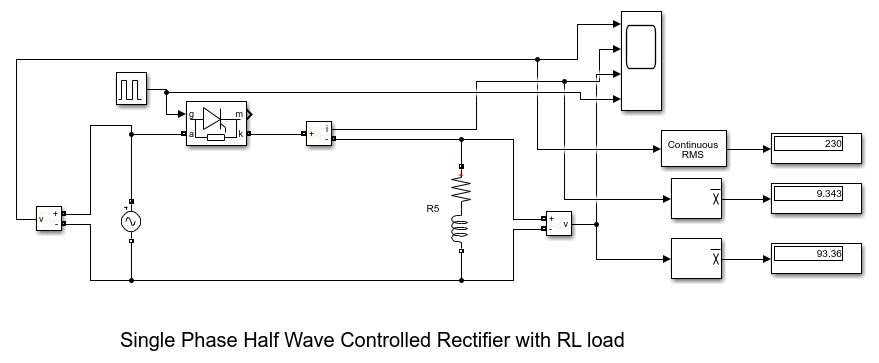
\includegraphics[width=0.7\textwidth]{images/experiment-1/circuit-diagram-simulation-06.png}
    \caption{Circuit used for simulation (Firing Angle = 30$ ^\circ $))}
    \label{Fig_simulation_circuit_single-phase-half-wave-controlled-rectifier-with-RL-load}
\end{figure}

\subsection{Components Required}

\begin{table}[h]
    \renewcommand{\arraystretch}{1.3}
    \label{table_components_required_circuit_6}
    \centering
    \begin{tabular}{|c|c|c|c|}
        \hline
        Sr. No & Parameters                     & Ratings            & Quantity \\
        \hline
        \hline
        1      & AC Single Phase Voltage Source & 230V ($ V_{rms} $) & 1        \\
        \hline
        2      & Resistor                       & 10$ \Omega $       & 1        \\
        \hline
        3      & Inductor                       & 10mH               & 1        \\
        \hline
        4      & Diode                          & -                  & 1        \\
        \hline
        5      & Voltmeter                      & -                  & 2        \\
        \hline
        6      & Ammeter                        & -                  & 1        \\
        \hline
        7      & Thyristor                      & -                  & 1        \\
        \hline
    \end{tabular}
    \caption{Components for Single Phase Half Wave Controlled Rectifier with RL load}

\end{table}




\subsection{Observations}

\begin{table}[h]
    \renewcommand{\arraystretch}{1.3}
    \label{table_observation_6}
    \centering
    \begin{tabular}{|c|c|c|}
        \hline
        Parameters                              & Theoretical Values & Simulation Values \\
        \hline
        \hline
        AC Input Voltage ($ V_{in,rms} $)       & 230V               & 230V              \\
        \hline
        Output Average Voltage ($ V_{o,avg} $)  & 96.6V              & 93.36V            \\
        \hline
        Output Average Current ($ I_{o,avg}  $) & 9.66A              & 9.343A            \\
        \hline
        AC Input Power ($ P_{AC}  $)            & 2214.44 (W)        & 2296 (W)          \\
        \hline
        DC Input Power ($ P_{DC}  $)            & 926.98 (W)         & 872.3 (W)         \\
        \hline
        Efficiency (\%)                         & 41.86              & 37.99             \\
        \hline
    \end{tabular}
    \caption{Observations for Single Phase Half Wave Controlled Rectifier with RL load}

\end{table}


Upon giving a firing gate pulse to the thyristor, the circuit starts conducting. As the load has an inductive component, the output current lags the output voltage. This causes the diode to conduct until the output current reaches zero, which results in the output voltage becoming negative during this time period. Once the output current becomes zero, the thyristor stops conducting and the output voltage also returns to zero. This operation is known as a half-wave uncontrolled rectifier.
rectifier with RL load is 37.99\%.


% \pagebreak

\subsection{Resultant Waveforms}

% figure that is centered on the page
\begin{figure}[h]
    \centering
    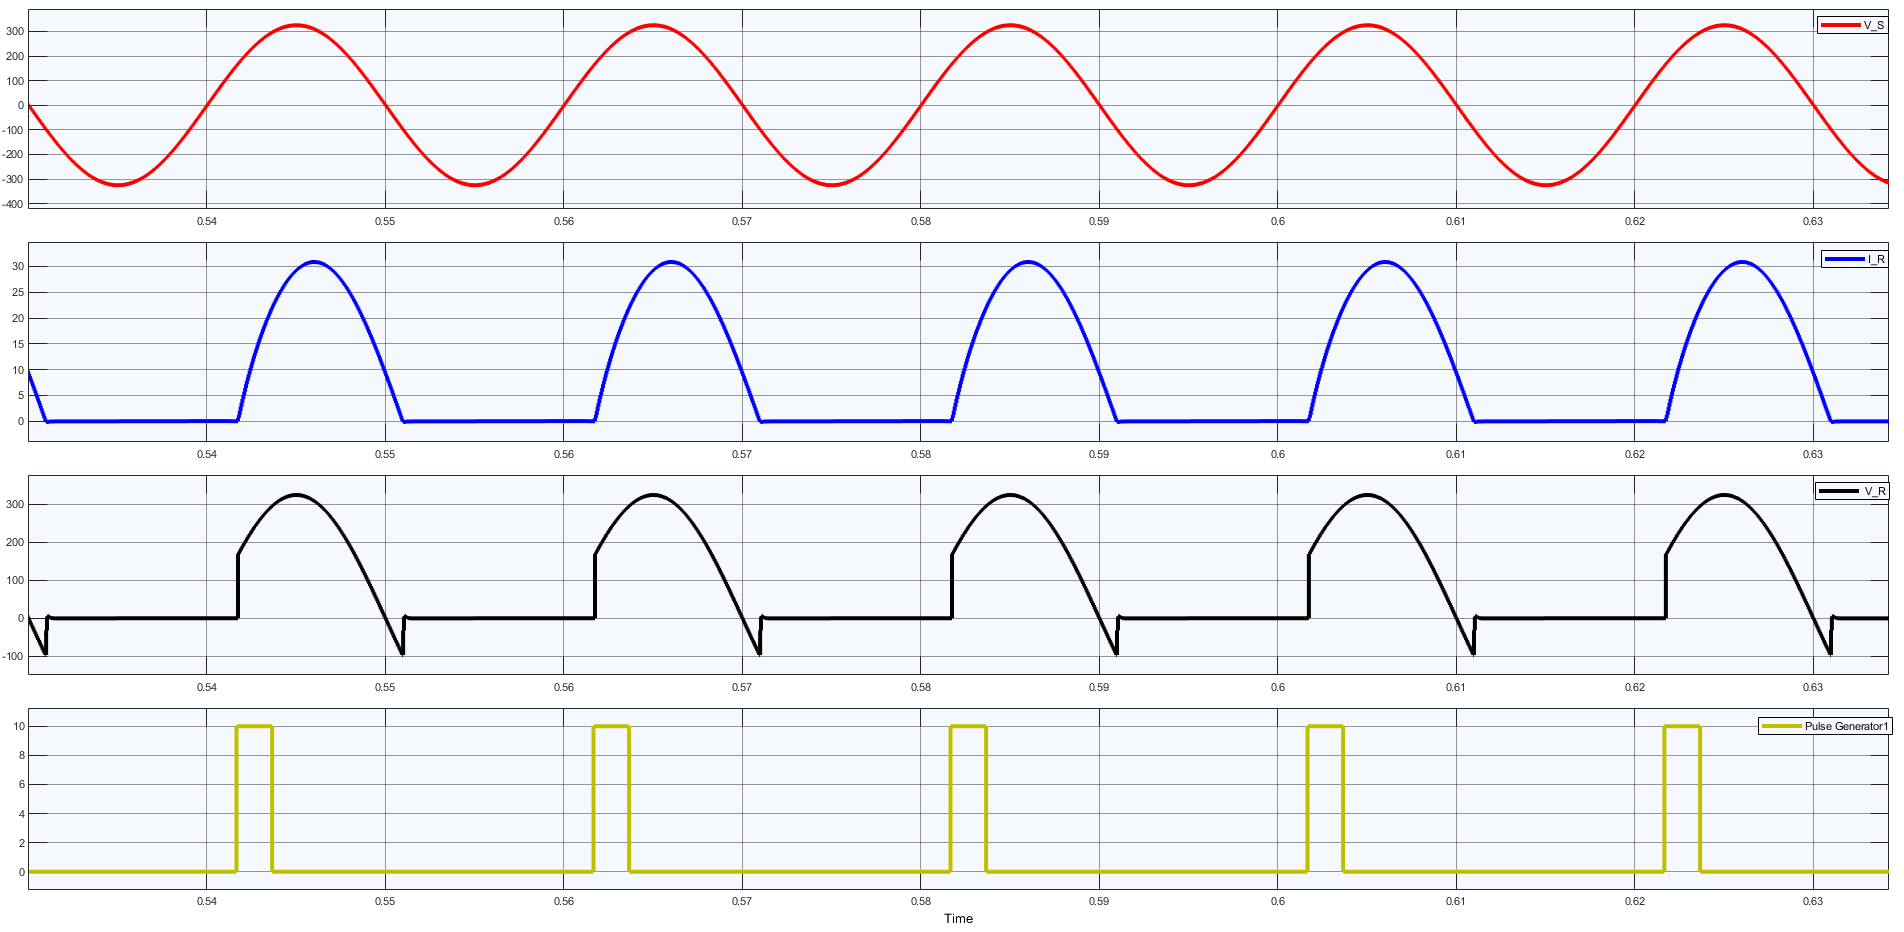
\includegraphics[width=1\textwidth]{images/experiment-1/circuit-scope-simulation-06.png}
    \caption{Scope Waveforms for Single Phase Half Wave Controlled Rectifier with RL load}
    \label{Fig_waveform_single-phase-half-wave-controlled-rectifier-with-RL-load}
\end{figure}

\pagebreak
